\section{Experiment}
\paragraph{}
This experiment followed strict patterns to ensure that it would not affect the servers of each of the tested solutions. No real data was used in the tests. Each solution got an account created and fake data inserted into it.


\subsection{Testing environment}
\paragraph{}
The research will be conducted within a client-server environment.

\subsubsection{Servers}
\paragraph{}
In this research we will be using five servers with the following specifications:\\~\\
\textbf{Physical server}
\begin{itemize}
	\item Intel Xeon processor
	\item 8GB ram
	\item SSD + HDD for storage
\end{itemize}

 Four physical servers we will be using each server to setup a separate service. Additional tools will be used, as well multiple logging and bench marking tools that allow us to keep a detailed log on the resource consumption and performance measurement. The fifth physical server is used for building the virtual setup.
 

\textbf{virtual server}
\paragraph{}
For the virtual server we will be using Xen 4.8.2 as hypervisor to implements the VMs. On top of the hypervisor there is a Dom0.

\paragraph{}
To test the solutions the following tools were used to setup a testing environment:
\begin{itemize}
    \item Ubuntu 16.04.2
    \begin{itemize}
        \item Virtual Box - 5.0.40
        \begin{itemize}
            \item Windows 7 and 10 x64 - Fully updated
            \begin{itemize}
                \item Process Explorer - 16.21
                \item Windows 7/10 SDK - 7.1/10.0.15063.400
                \item Proxifier - 3.31
            \end{itemize}
        \end{itemize}
        \item Burp Suite - 1.7.23
        \item Apktool - 2.2.2
        \item Dex2jar - Commit dd9d722
        \item Jd\_Gui - Commit acd511f
    \end{itemize}
    \item Android - 7.1.2
    \begin{itemize}
        \item Proxydroid - 2.7.7
    \end{itemize}
\end{itemize}

\begin{figure}[H]
    \centering
    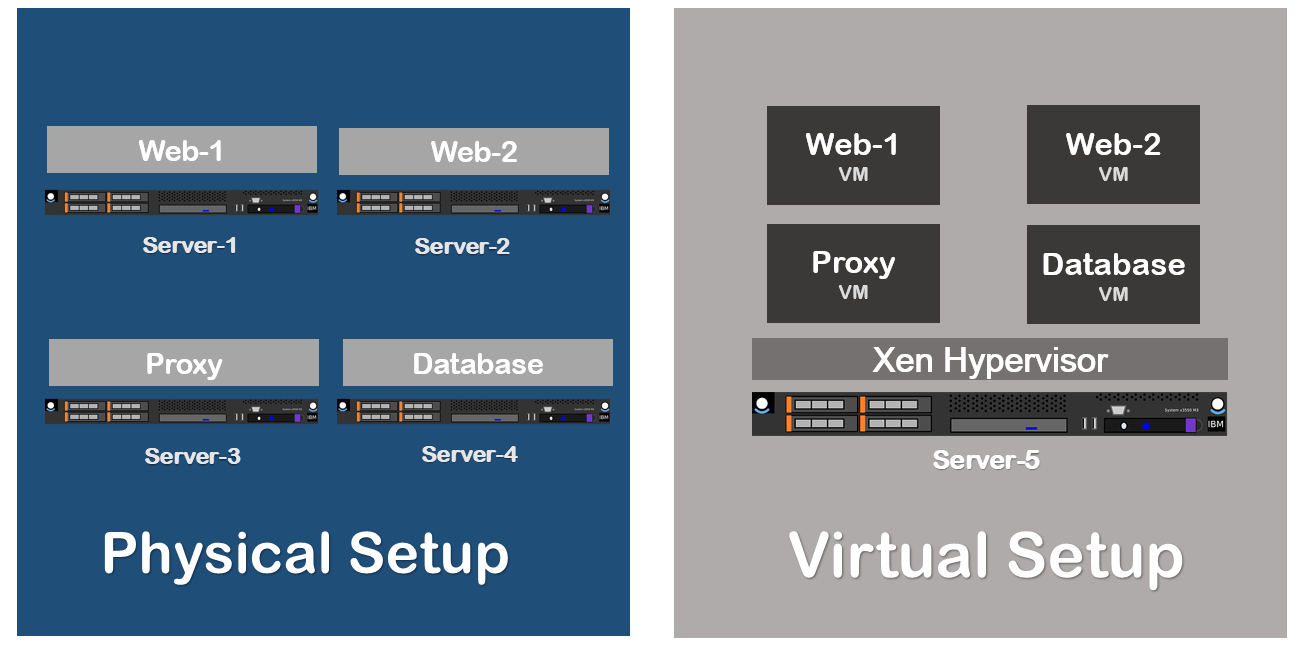
\includegraphics[width=14cm]{Pictures/setup.PNG}
    \caption{Test Environment Setup}
    \label{fig:QQ3}
\end{figure}

\textbf{\textit{Figure 3}} above illustrates both the physical and virtual setups environment, in addition to each service that run on which server.


\subsection{Tool}

%%tools we use


\clearpage
\subsection{Methodology}
\paragraph{}
In this project we followed a methodology that starts from basic tests to increasingly complex ones on both virtual and physical servers. The steps we followed were:
\begin{itemize}
    \item \textbf{Basic setup tests:}
 In the basic setup tests we used only the Apache HTTP server benchmarking tool to experiment the web server alone by itself without the complete setup as illustrated in the \textbf{\textit{figure 1}}. 
 We targeted only the static web page of our osCommerce store.
 \begin{figure}[H]
    \centering
    
\includegraphics[width=6cm]{Pictures/simple.PNG}
    \caption{Basic Setup Test Methodology}
    \label{fig:QQ3}
\end{figure}
   
    
    
    \item \textbf{Full setup tests:}
 For the complete setup test we used both the Apache HTTP server benchmarking tool and Paessler webserver Stress tool to experiment the complete setup environment which includes proxy, web, and database servers as shown in \textbf{\textit{figure 2}}. 
 We targeted the proxy server which acts as load balancer between our two webservers. And these two webservers interact directly with the database server. Which leads to a complete setup tests.   
 \begin{figure}[H]
    \centering
    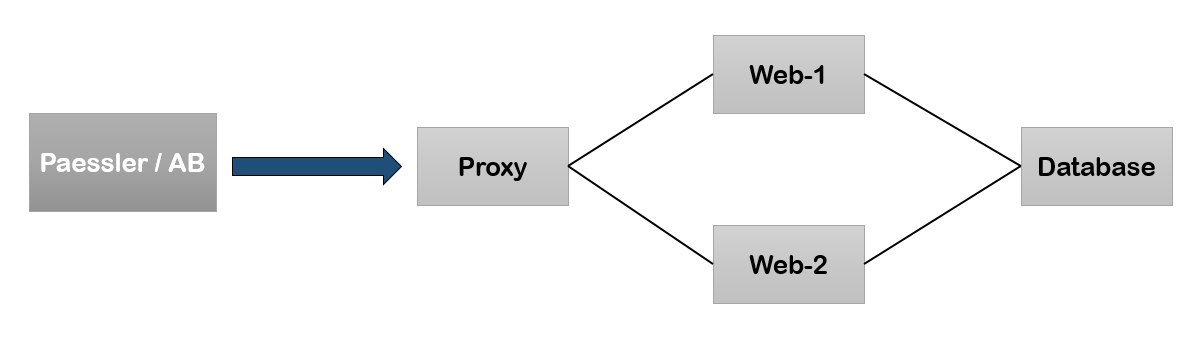
\includegraphics[width=12cm]{Pictures/complex.PNG}
    \caption{Full Setup Test Methodology}
    \label{fig:QQ3}
\end{figure}

\end{itemize}

\subsubsection{Paessler Webserver Stress Tool}
\paragraph{}

\textbf{ALEXANDER write here how we adjust the Paessler tool ( number of users and etc..) also include screenshot about how we customized the URLs and etc}

\subsubsection{Measuring requests \& transferred data}
\paragraph{}

\textbf{\textit{figure 3}} \& \textbf{\textit{figure 4}} below show the number of open requests as well as the number of sent and received requests in comparison with the network traffic on both the virtual and physical setups:
 

 \begin{figure}[H]
    \centering
    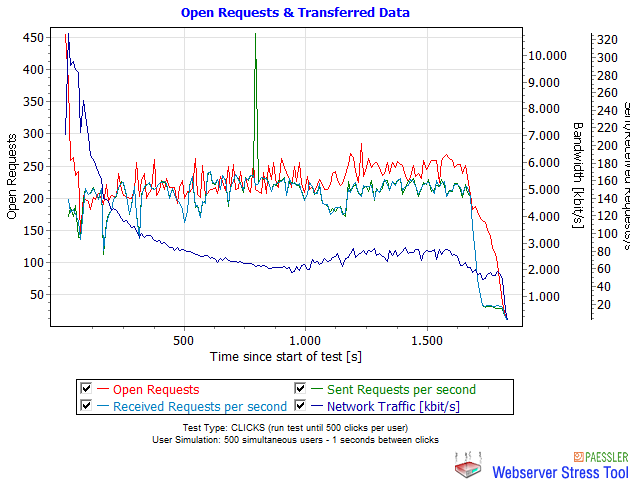
\includegraphics[width=10cm]{Pictures/graph6hw.png}
    \caption{Requests \& Transferred Data for Physical Setup}
    \label{fig:QQ3}
\end{figure}
   
 
\begin{figure}[H]
    \centering
    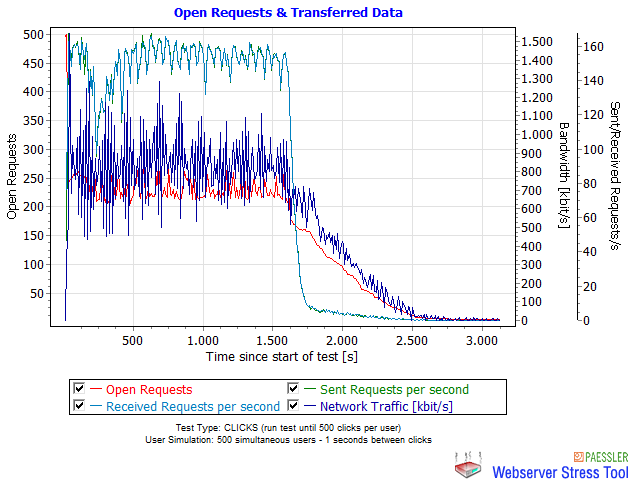
\includegraphics[width=10cm]{Pictures/graph6vm.png}
    \caption{Requests \& Transferred Data for Virtual Setup}
    \label{fig:QQ3}
\end{figure} 


\paragraph{}
\textbf{ALEXANDER also write here small conclusion about these two graphs}


\subsubsection{Measuring transferred Data \& system Memory \& CPU load}
\paragraph{}

\textbf{\textit{figure 5}} \& \textbf{\textit{figure 6}} describe the measurement for vital parameters of the machine it runs on. It can be helpful to find out if the limits of the test client have been reached. both the virtual and physical setups:
 

 \begin{figure}[H]
    \centering
    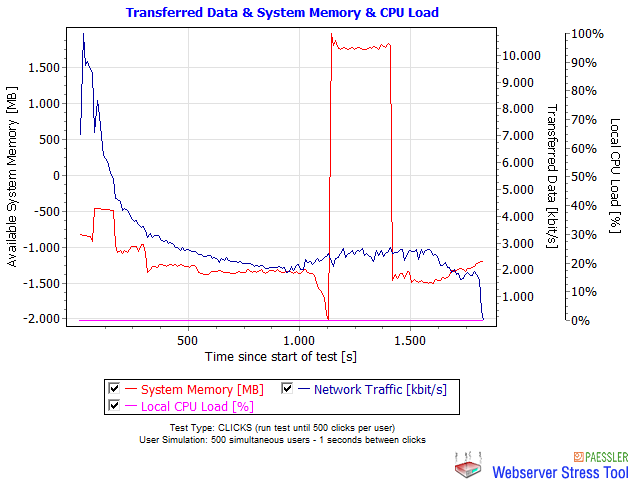
\includegraphics[width=10cm]{Pictures/ph1.png}
    \caption{Transferred Data \& System Memory \& CPU Load for Physical Setup}
    \label{fig:QQ3}
\end{figure}
   
 
\begin{figure}[H]
    \centering
    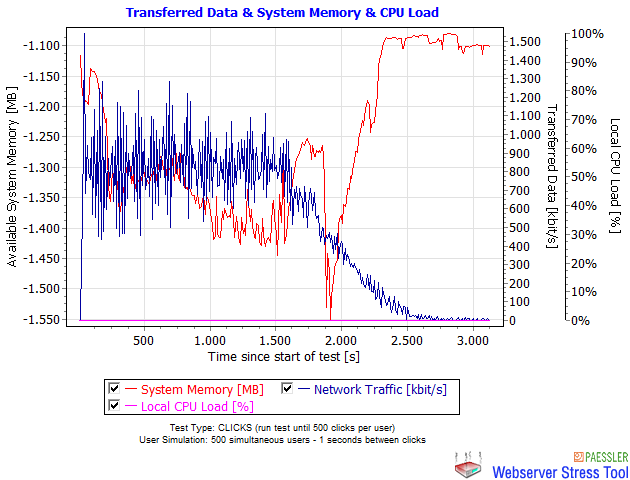
\includegraphics[width=10cm]{Pictures/vm1.png}
    \caption{Transferred Data \& System Memory \& CPU Load for Virtual Setup}
    \label{fig:QQ3}
\end{figure} 


\paragraph{}
\textbf{ALEXANDER also write here small conclusion about these two graphs}



\subsubsection{Measuring Click Time, Hits/s \& Clicks/s}
\paragraph{}

\textbf{\textit{figure 6}} \& \textbf{\textit{figure 7}} illustrate the average time a user waited for his request to be processed (including redirects, images, frames, etc., if enabled), the hits per second, and the users per clicks. 

 \begin{figure}[H]
    \centering
    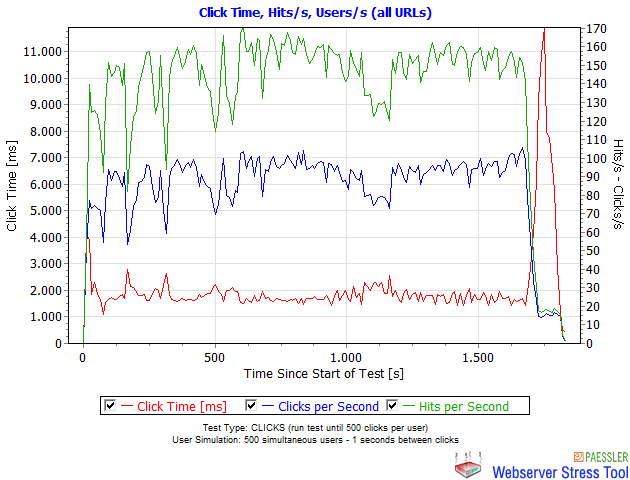
\includegraphics[width=10cm]{Pictures/ph2.png}
    \caption{Click Time, Hits/s \& Clicks/s for Physical Setup}
    \label{fig:QQ3}
\end{figure}
   
 
\begin{figure}[H]
    \centering
    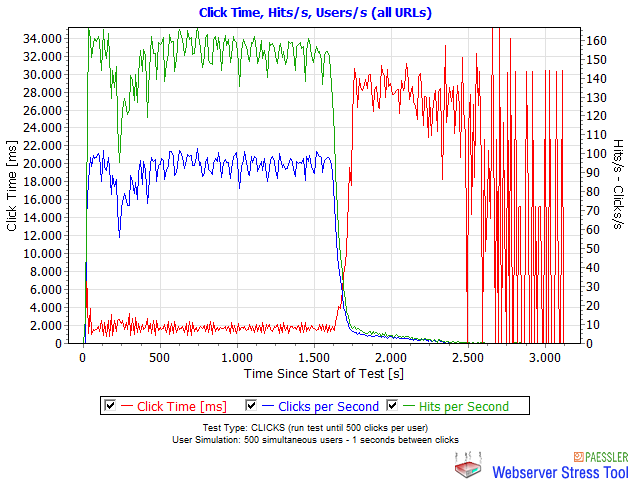
\includegraphics[width=10cm]{Pictures/vm2.png}
    \caption{Click Time, Hits/s \& Clicks/s for Virtual Setup}
    \label{fig:QQ3}
\end{figure} 


\paragraph{}
We can see that with 500 users the two lines for “clicks per second” (blue) and “hits per second” (green) differ more and more. The reason is that hits includes requests that produce errors, but clicks are only calculated from the requests that were successful.




\subsubsection{Apache Benchmark}

NOTE: Below should be an image with the test 
%%                  > WEB 1 \
%%    AB to Proxy  <         > Database 
%%                  > WEB 2 /

NOTE: Below should be an image with the test 
%%      AB to      > WEB 1 